\documentclass{article}
\usepackage[margin=1in]{geometry}

\usepackage{graphicx, booktabs, caption, mathtools, amsfonts, amsthm, soul}
\newtheorem{theorem}{Theorem}[section]
\newtheorem{lemma}[theorem]{Lemma}
\newtheorem{corollary}[theorem]{Corollary}
\newtheorem{example}[theorem]{Example}
\newtheorem{remark}[theorem]{Remark}
\theoremstyle{definition}
\newtheorem{definition}{Definition}[section]
% qed symbo
\renewcommand\qedsymbol{$\blacksquare$}

% no indent
\setlength{\parindent}{0pt}

\usepackage{tikz}
\usetikzlibrary{calc,shapes.geometric, decorations.markings}


\title{\LARGE MATH 311 Final Summary \\[1em] \normalsize Eddie Guo \\ \today}
\author{}
\date{}

\begin{document}
\maketitle

% Harmonic Functions
\section{Harmonic Functions}

\begin{definition}
    (Harmonic functions). Let $D \subset \mathbb{R}^2$ be a domain and let $h(x, y)$ be a continuous real-valued function with continuous partial derivatives. Then $h$ is harmonic on $D$ if $h$ satisfies Laplace's equation, $h_{xx} + h_{yy} = 0$.
\end{definition}

\begin{theorem}
    Let $f(z) = \mu + i \nu$ be analytic on $D$. Then $\mu$ and $\nu$ are harmonic on $D$.
\end{theorem}

\begin{example} \normalfont
    Given $f(z) = 1/z$ is analytic on $D := \mathbb{C} \setminus \{0\}$,
    \begin{equation*}
        f(z) = \frac{\bar{z}}{z \bar{z}} = \underbrace{\frac{x}{x^2+y^2}}_\mu - i \underbrace{\frac{y}{x^2+y^2}}_\nu
    \end{equation*} \vspace{-2em}

    $\mu$ and $\nu$ are harmonic on $D$.
\end{example}

\begin{example} \normalfont
    Let $\mu(x, y) = 2x(1-y)$. Find a real function $\nu(x, y)$ on $\mathbb{R}^2$ s.t. $f(z) = \mu + i \nu$ is entire (i.e., find the harmonic conjugate of $\mu$).
    \begin{align*}
        \mu_x &= 2(1-y) = \nu_y \implies \nu = 2y-y^2 + C(x) \implies \nu_x = C'(x) \\
        -\mu_y &= 2x = \nu_x = C'(x) \implies C(x) = x^2 \implies \nu = 2y-y^2+x^2 \\
        f(z) &= 2(1-y) + i (2y -y^2 + x^2) \text{ is entire.}
    \end{align*}
\end{example}


% Conformal Maps
\section{Conformal Maps}

\begin{definition}
    Let $D$ be a domain, $p \in D$, and $f: D \mapsto \mathbb{C}$. The function $f$ is said to be conformal if it preserves angles at $p$. Furthermore, $f$ is conformal on $D$ if $f$ is conformal $\forall p \in D$.
\end{definition}

\begin{theorem}
    Suppose $f$ is analytic on $D$, $p \in D$, and $f'(p) \neq 0$, $\forall p \in D$. Then $f$ is conformal on $D$.
\end{theorem}

\begin{example} \normalfont
    Let $f(z) = az+b,\ a \neq 0$. Then $f'(z) = a \neq 0$, so $f$ is conformal on $\mathbb{C}$.
\end{example}

\begin{example} \normalfont
    Let $f(z) = z^2 \implies f'(z) = 2z \neq 0 \iff z \neq 0$, so $f$ is conformal on $\mathbb{C} \setminus \{0\}$.
\end{example}

\begin{theorem}
    Let $D \subseteq \mathbb{C}$ be a domain and $w$ be a non-constant function that is analytic at $p \in \mathbb{C}$. If
    \begin{equation*}
        w = w(p) + a_m (z-p)^m + (\text{higher order terms})
    \end{equation*}
    where $m$ is the smallest integer for which $f^{(n)}(p) \neq 0$, then the effect of the angle $\theta$ is $m\theta$.
\end{theorem}

\begin{example} \normalfont
    Let $f(z) = z^2$. Then $f'(z) = 2z + 2 \neq 0$, so $f$ is conformal on $\mathbb{C} \setminus \{0\}$. Furthermore, $f''(z) = 2 \neq 0$ so the effect is $\theta \mapsto 2 \theta$ at $z = 0$.
\end{example}


% Contour Integrals
\section{Contour Integrals}

\begin{definition}
    Let $z(t): [a, b] \mapsto \mathbb{C}$ and $C: z([a, b])$ be the piecewise differentiable curve $C$ parameterized by $z(t)$. Let $f(z)$ be a complex-valued function defined on $C$. Then the contour integral is defined as
    \begin{equation*}
        \int_C f(z)\ dz := \int_a^b f(z(t)) z'(t)\ dt
    \end{equation*}
    If $C = C_1 + C_2 + \cdots C_N$, then
    \begin{equation*}
        \int_C f(z)\ dz = \sum_{i=1}^N \int_{C_i} f(z)\ dz
    \end{equation*}
\end{definition}

\begin{example} \normalfont
    Let $f(z) = \begin{cases}
        1, & y > 0 \\ 4y, & y < 0
    \end{cases},\ z(t) = t + it^3: [-1, 1] \mapsto \mathbb{C}$. Evaluate the integral $\int_C f(z)\ dz$.

    \begin{equation*}
        \int_C f(z)\ dz = \int_{-1}^0 1(1+3it^2)\ dt + \int_0^1 4t^3 (1+3it^2)\ dt = 4+i
    \end{equation*}
\end{example}

\begin{definition}
    If a curve $C$ is parameterized by $z(t): [a, b] \mapsto C$, then the equivalent curve with opposite orientation is $C^-$ parameterized by $z(t) := z(-t): [-b, -a] \mapsto C^-$. Furthermore,
    \begin{equation*}
        \int_C f(z)\ dz = -\int_{C^-} f(z)\ dz
    \end{equation*}
    Parameterizing straight lines: Let $P, Q \in \mathbb{C}$. Then $z(t) = Q + t(P-Q): [0, 1] \mapsto C$ where $z(0) = Q$, and $z(1) = P$ is a straight line connecting $P$ and $Q$.
\end{definition}


% Section
\section{Important Theorems}

\begin{theorem}
    \hl{(Cauchy-Goursat theorem).} Let $C$ be a simple, closed curve and $f(z)$ be an analytic function on $C$ and its interior. Then
    \begin{equation*}
        \int_C f(z) = 0
    \end{equation*}
\end{theorem}

\begin{example} \normalfont
    By the Cauchy-Goursat theorem,
    \begin{equation*}
        \int_{|z+1| = \pi} \frac{\sin z^8 - 14 \cos^2 (5z) + e^{e^z}}{e^{z^2-4z^3+4}} = 0
    \end{equation*}
\end{example}

\begin{theorem}
    (ML inequality). Let $f(z) \leq M$ and $L = \int_C |dz|$. Then
    \begin{equation*}
        \left| \int_C f(z)\ dz \right| \leq ML
    \end{equation*}
\end{theorem}

\begin{example} \normalfont
    \begin{align*}
        \left| \int_{|z|=2} \frac{z^3+z-2}{z^2-1}\ dz \right| &\leq \int_{|z|=2} \left| \frac{z^3+z-2}{z^2-1} \right|\ |dz| \\
        &\leq \int_{|z|=2} \frac{|z|^3 + |z| + 2}{| |z|^2 - 1 |}\ |dz|,\quad \text{by the triangle inequality} \\
        &= 4(2 \pi \times 2)\\
        &= 16 \pi
    \end{align*}
\end{example}

\begin{example} \normalfont
    Let $C$ be a simple, closed curve containing 0 in its interior. Let $f(z) = z^n$. Then
    \begin{equation*}
        \oint_C z^n\ dz = \begin{cases}
            2 \pi i, & n = -1 \\
            0, & \text{otherwise}
        \end{cases}
    \end{equation*}
\end{example}

\begin{theorem}
    \hl{(Cauchy integral formula).} Let $C$ be a simple, closed curve with point $p$ in its interior. Let $f$ be analytic on and inside $C$. Then
    \begin{equation*}
        f(p) = \frac{1}{2 \pi i} \int_C \frac{f(z)}{z-p}
    \end{equation*}
    Furthermore,
    \begin{equation*}
        f^{(n)}(p) = \frac{n!}{2 \pi i} \oint_C \frac{f(z)}{(z-p)^{n+1}}\ dz
    \end{equation*}
\end{theorem}

\begin{example} \normalfont
    Evaluate
    \begin{equation*}
        \int_C \frac{e^{iz}}{(z-1)^2}\ dz,\quad \text{where $C: |z+i| = 10$}
    \end{equation*}
    Note that $f(z) = e^{iz}$, $p=1$, and $n=1$.
    \begin{equation*}
        \int_C \frac{e^{iz}}{(z-1)^2}\ dz = \frac{2 \pi i}{1!} \frac{d}{dz}(e^{iz}) |_{z=1} = -2 \pi e^i
    \end{equation*}
\end{example}

\begin{example} \normalfont
    Compute
    \begin{equation*}
        \oint_C \frac{dz}{z^3 (z+4)}
    \end{equation*}
    for (a) $|z|=2$, (b) $|z+3|=2$, (c) $|z| = 100$, and (d) $|z-100| = 1$.

    (a) $f(z) = 1/(z+4)$, $p=0$, and $n=2$
    \begin{equation*}
        \oint_C \frac{dz}{z^3 (z+4)} = \frac{2 \pi i}{2!} f''(0) = \frac{\pi i}{32}
    \end{equation*}

    (b) $f(z) = 1/z^3$, $n=0$, and $p=-4$.
    \begin{equation*}
        \oint_C \frac{dz}{z^3 (z+4)} = \frac{2 \pi i}{0!} f(-4) = -\frac{\pi i}{32}
    \end{equation*}

    (c) Add answers in (a) and (b) to get $0$. (d) 0 by Cauchy-Goursat.
\end{example}


% Standard Theorems in Complex Analysis
\section{Standard Theorems in Complex Analysis}

\begin{theorem}
    If $f$ is analytic, $f'$ is also analytic.
\end{theorem}

\begin{theorem}
    (Liouville's theorem). The only bounded entire functions are constants.
\end{theorem}

\begin{theorem}
    (Maximum modulus principle). Let $f$ be analytic on domain $D \subset \mathbb{C}$ and fix $p \in D$. If $|f(z)| \leq |f(p)|,\ \forall z \in D$, then $f$ is constant on $D$. \vspace{1em}

    Variant: Assume $D$ is bounded, $f$ is anaytic on $D$, and $f$ extends to a continuous function on $\bar{D}$. If $f(z)$ non-constant on $D$, then $|f(z)|$ obtains its max on $\partial D$.
\end{theorem}

\begin{theorem}
    (Fundamental theorem of algebra). Let $p(z) \in \mathbb{C}$ be a polynomial of degree $\geq 1$. Then $\exists r \in \mathbb{C}$ s.t. $p(r) = 0$.
\end{theorem}

\begin{theorem}
    (Morera's theorem). Let $D \subseteq \mathbb{C}$ be a domain and $f(z)$ be a continuous complex-valued function on $D$. Suppose that
    \begin{equation*}
        \int_C f(z)\ dz = 0,\quad \forall C \subseteq D
    \end{equation*}
    Then $f(z)$ is analytic on $D$.
\end{theorem}


% Power Series
\section{Power Series}

\begin{definition}
    (Radius of convergence). If both limits exist, they will yield the same $R$.
    \begin{equation*}
        R = \lim_{n \to \infty} \left| \frac{a_n}{a_{n+1}} \right|, \quad R = \lim_{n \to \infty} \frac{1}{\sqrt[n]{|a_n|}}
    \end{equation*}
\end{definition}

\begin{example} \normalfont
    Compute radius of convergence for $\sum_{n=1}^\infty \frac{n5^n}{i} (z+2i)^n$
    \begin{equation*}
        R = \lim_{n \to \infty} \left| \frac{n 5^n}{i} \times \frac{i}{(n+1) 5^{n+1}} \right| = \frac{1}{5} \implies |z+2i| < \frac{1}{5}
    \end{equation*}
\end{example}

\begin{example} \normalfont
    Compute radius of convergence for $\sum_{n=1}^\infty \frac{(2z+3i)^n}{n}$.
    \begin{align*}
        &\sum_{n=1}^\infty \frac{[2(z+3i/2)]^n}{n} = \sum_{n=1}^\infty \frac{2^n}{n} \left( z + \frac{3i}{2} \right)^n \\
        R &= \lim_{n \to \infty} \frac{1}{\sqrt[n]{|2^n/n|}} = \lim_{n \to \infty} \frac{1}{2(1/n)^{1/n}} = \frac{1}{2}
    \end{align*}
\end{example}

\begin{example} \normalfont
    Compute radius of convergence for $\sum_{n=0}^\infty \frac{2^n i}{z^n}$.
    \begin{equation*}
        \lim_{n \to \infty} = \frac{1}{\sqrt[n]{2^n i}} = \frac{1}{2}
    \end{equation*}
    Converges if $|z| > 1/2$ and diverges if $|z| < 1/2$.
\end{example}


% Laurent Series
\section{Laurent Series}

\begin{definition}
    A Laurent series centered at $p \in \mathbb{C}$ is the sum
    \begin{equation*}
        \sum_{n=-\infty}^\infty c_n (z-p)^n = \sum_{n=1}^\infty \frac{b_n}{(z-p)^n} + \sum_{n=0}^\infty a_n (z-p)^n
    \end{equation*}
    where $b_n = c_{-n}$ for $n \geq 1$ and $a_n = c_n$ for $n \geq 0$.
\end{definition}

\begin{theorem}
    If $\exists r, R \in [0, \infty]$ st $\sum_{n=-\infty}^\infty c_n (z-p)^n$ defines an analytic function on $r < |z-p| < R$, then
    \begin{align*}
        R = \lim_{n \to \infty} \frac{1}{\sqrt[n]{|a_n|}} \quad \text{or} \quad R = \lim_{n \to \infty} \left| \frac{a_n}{a_{n+1}} \right| \\
        r = \lim_{n \to \infty} \sqrt[n]{|a_n|} \quad \text{or} \quad r = \lim_{n \to \infty} \left| \frac{b_{n+1}}{b_n} \right| \\
    \end{align*}
\end{theorem}

\begin{theorem}
    Assume that $0 \leq r < R \leq \infty$ and $f(z)$ is analytic on $r < |z-p| < R$. Then $f(z)$ is equal to a Laurent series on this annular region. Then the coefficients of the series are
    \begin{align*}
        a_n &= \frac{1}{2 \pi i} \oint_{|z-p| = R'} \frac{f(z)}{(z-p)^{n+1}}\ dz \\
        b_n &= \frac{1}{2 \pi i} \oint_{|z-p| = r'} f(z) (z-p)^{n-1}\ dz
    \end{align*}
\end{theorem}

\begin{remark}
    \hl{(Geometric series).} If $\exists$singularity at $z=p$, then the Laurent expansion about $p$ is
    \begin{equation*}
        \begin{cases}
            \displaystyle \frac{1}{1-cw} = \sum_{n=0}^\infty (cw)^n, & |w| < \frac{1}{|c|} \\
            \displaystyle \frac{1}{1-c/w} = \sum_{n=0}^\infty \left( \frac{c}{w} \right)^n, & |w| > |c|
        \end{cases}
    \end{equation*}
    where $p$ lies on $|z| = c$ (think radius of convergence).
\end{remark}

\begin{example} \normalfont
    \hl{Show that the Laurent series for}
    \begin{equation*}
        f(z) = \frac{5z}{z^2+z-6}
    \end{equation*}
    in the annular region $1 < |z-1| < 4$ is given by
    \begin{equation*}
        \sum_{n=1}^\infty \frac{2}{(z-1)^2} + \sum_{n=0}^\infty \frac{3(-1)^n}{4^{n+1}} (z-1)^n
    \end{equation*}
    Let $w=z-1$ and observe that $z^2+z-6 = (z+3)(z-2) = (w+4)(w-1)$. Hence
    \begin{equation*}
        \frac{5z}{z^2+z-6} = \frac{5(w+1)}{(w+4)(w-1)} = \frac{3}{w+4} + \frac{2}{w-1}
    \end{equation*}
    On $|w| > 1$, we have:
    \begin{equation*}
        \frac{2}{w-1} = \frac{2}{w}\left( \frac{1}{1-1/w} \right) = \frac{2}{w} \sum_{n=0}^\infty \frac{1}{w^n} = \sum_{n=0}^\infty \frac{2}{w^{n+1}} = \sum_{n=1}^\infty \frac{2}{w^n} = \sum_{n=1}^\infty \frac{2}{(z-1)^n}
    \end{equation*}
    On $|w|<4$ we have:
    \begin{equation*}
        \frac{3}{w+4} = \frac{3}{4} \left( \frac{1}{1 + w/4} \right) = \frac{3}{4} \sum_{n=0}^\infty \frac{(-1)^n}{4^n} w^n = \sum_{n=0}^\infty \frac{3(-1)^n}{4^{n+1}} w^n = \sum_{n=0}^\infty \frac{3(-1)^n}{4^{n+1}} (z-1)^n
    \end{equation*}
    Thus on $1 < |w| = |z-1| < 4$:
    \begin{equation*}
        \frac{5}{z^2+z-6} = \sum_{n=1}^\infty \frac{2}{(z-1)^n} + \sum_{n=0}^\infty \frac{3(-1)^n}{4^{n+1}} (z-1)^n
    \end{equation*}
\end{example}

\begin{theorem}
    (Riemann extension theorem). Suppose that $f(z)$ is both analytic and bounded on $0 < |z-p| < R$. Then $f(z)$ extends analytically to $z = p$.
\end{theorem}

\begin{theorem}
    \hl{(Taylor series).} If $b_n = 0, \forall n \geq 1$, then
    \begin{equation*}
        f(z) = \sum_{n=0}^\infty \frac{f^{(n)} (p)}{n!} (z-p)^n
    \end{equation*}
\end{theorem}

\begin{example} \normalfont \vspace{-1em}
    \begin{align*}
        \sin z &= \sum_{n=0}^\infty \frac{(-1)^n z^{2n+1}}{(2n+1)!}, \quad \cos z = \sum_{n=0}^\infty \frac{(-1)^n z^{2n}}{(2n)!} \\
        \sinh z &= \sum_{n=0}^\infty \frac{z^{2n+1}}{(2n+1)!}, \quad \cosh z = \sum_{n=0}^\infty \frac{z^{2n}}{(2n)!}
    \end{align*}
\end{example}

\begin{example} \normalfont
    Compute the Taylor series for $f(z) = 1/(1+z)^2$.
    \begin{align*}
        F(z) &= \int \frac{dz}{(1+z)^2} = -\frac{1}{1+z} = - \sum_{n=0}^\infty (-1)^n z^n = \sum_{n=0}^\infty (-1)^{n+1} z^n \\
        f(z) &= F'(z) = \sum_{n=1}^\infty (-1)^{n+1} n z^{n-1} = \sum_{n=0}^\infty (-1)^n (n+1) z^n
    \end{align*}
\end{example}

\begin{example} \normalfont
    Compute the Taylor series for $f(z) = \log \frac{1+z}{1-z}$ on the branch where $\log 1 = 0$.
    \begin{align*}
        f(z) &= \log(1+z) - \log(1-z) \implies f'(z) = \frac{1}{1+z} + \frac{1}{1-z} = \frac{2}{1-z^2} = 2 \sum_{n=0}^\infty z^{2n} \\
        f(z) &= \int 2 \sum_{n=0}^\infty z^{2n}\ dz = 2 \sum_{n=0}^\infty \frac{z^{2n+1}}{2n+1}
    \end{align*}
\end{example}


% Isolated Singularities
\section{Isolated Singularities}

\begin{definition}
    Given an analytic function $f(z)$ on $0 < |z-p| < R \leq \infty$,
    \begin{equation*}
        f(z) = \sum_{n=1}^\infty \frac{b_n}{(z-p)^n} + \sum_{n=0}^\infty a_n (z-p)^n
    \end{equation*}
    Consider the point $p$. The function $f(z)$ has a
    \begin{enumerate}
        \item \hl{Removeable singularity} at $p$ if there is no principal part ($b_n = 0$).
        \item \hl{Pole singularity} at $p$ if $\exists m \geq 1$ s.t. $b_n = 0,\ \forall n > m,\ b_n \neq 0$ for some $n$ (truncated principal part).
        \item \hl{Essential singularity} at $p$ if $b_n \neq 0,\ \forall n \geq 1$.
    \end{enumerate}
\end{definition}

\begin{example} \normalfont
    (Removeable singularity). $f(z) = \sin z / z$.
    \begin{equation*}
        \frac{\sin z}{z} = \frac{1}{z} \sum_{n=0}^\infty \frac{(-1)^n z^{2n+1}}{(2n+1)!} = \sum_{n=0}^\infty \frac{(-1)^n z^{2n}}{(2n+1)!}
    \end{equation*}
\end{example}

\begin{example} \normalfont
    (Pole singularity). $f(z) = \cos z / z$.
    \begin{equation*}
        \frac{\cos z}{z} = \frac{1}{z} \sum_{n=0}^\infty \frac{(-1)^n z^{2n}}{(2n)!} = \frac{1}{z} + \sum_{n=1}^\infty \frac{(-1)^n z^{2n-1}}{(2n)!}
    \end{equation*}
\end{example}

\begin{example} \normalfont
    (Essential singularity). $f(z) = e^{1/z}$.
    \begin{equation*}
        e^{1/z} = \sum_{n=0}^\infty \frac{1}{n! z^n} = 1 + \sum_{n=1}^\infty \frac{1}{n!z^n}
    \end{equation*}
\end{example}

\begin{theorem}
    (Classifying singularities).
    \begin{enumerate}
        \item $p$ is a removeable singularity $\iff \lim_{z \to p} f(z) \in \mathbb{C}$ exists.
        \item $p$ is a pole singularity $\iff \lim_{z \to p} f(z) = \infty$.
        \item $p$ is an essential singularity $\iff \lim_{z \to p} f(z)$ DNE.
    \end{enumerate}
\end{theorem}

% Zeroes of an Analytic Function
\section{Zeroes of an Analytic Function}

\begin{definition}
    Let $f(z)$ be analytic on $|z-p| < R$. Assume $f(z) \neq 0$ on $|z-p| < R$ and $f(p) = 0$. By Taylor, $f(z) = a_n (z-p)^n + a_{n+1} (z-p)^{n+1} + \cdots$ where $a_n \neq 0$ for some $n \geq 1$. We say that $p$ is a zero of $f(z)$ of order $n$.
\end{definition}

\begin{theorem}
    Suppose $f(z)$ is analytic on a domain $D$ and for some $p \in D$, we have $f^{(n)}(p) = 0,\ n \in \mathbb{Z}$. Then $f(z) = 0$ on $D$.
\end{theorem}

\begin{theorem}
    Let $f(z) = \frac{b_M}{(z-p)^M} + \frac{b_{M-1}}{(z-p)^{M-1}} + \cdots + \frac{b_1}{z-p},\ b_M \neq 0$ be analytic. Then $f$ has a pole of order $M$ at $p \iff h:=1/f$ has a zero of order $M>0$ at $p$.
\end{theorem}

% Residues
\section{Residues}

\begin{theorem}
    (Finding residues). Let $b_1 = \text{Res}_p f(z)$ be a residue of $f(z)$ at the point $p$.
    \begin{enumerate}
        \item Removeable singularities: $\text{Res}_p f(z) = 0$.
        \item \hl{Simple pole:} Find the Laurent series then find $b_1$ OR compute $b_1 = \lim_{z \to p} f(z)(z-p)$.
        \item \hl{Pole of order $m$:}
        \begin{equation*}
            b_1 = \lim_{z \to p} \frac{1}{(m-1)!} \frac{d^{m-1}}{dz^{m-1}} \left[ f(z) (z-p)^m \right]
        \end{equation*}
    \end{enumerate}
\end{theorem}

\begin{example} \normalfont
    $f(z) = e^{1/z}$.
    \begin{equation*}
        e^{1/z} = \sum_{n=0}^\infty \frac{1}{n! z^n} = 1 + \frac{1}{z} + \sum_{n=2}^\infty \frac{1}{n! z^n} \implies \text{Res}_0 e^{1/z} = 1
    \end{equation*}
\end{example}

\begin{example} \normalfont
    $f(z) = e^{1/z^2}$
    \begin{equation*}
        e^{1/z^2} = 1 + \frac{1}{z^2} + \frac{1}{2z^4} + \cdots \implies \text{Res}_0 e^{1/z^2} = 0
    \end{equation*}
\end{example}

\begin{example} \normalfont
    Let $f(z) = 1/(z^2+1)$. Find the residue at $z = i$.
    
    Set $g(z) = 1/(z+i) \implies g(i) = 1/(2i) \neq 0, f(z) = g(z) / (z-i)$. By Taylor,
    \begin{align*}
        g(z) &= g(i) + g'(i) (z-i) + \frac{g''(i)}{2!} (z-i) + \cdots \\
        f(z) &= \frac{g(z)}{z-i} = \frac{g(i)}{z-i} + g'(i) + \frac{g''(i)}{2!} (z-i) + \cdots \implies \text{Res}_i f(z) = g(i) = \frac{1}{2i}
    \end{align*}
\end{example}

\begin{example} \normalfont
    $f(z) = \frac{e^z+1}{(z-\pi)^3}$. Compute $\text{Res}_\pi f(z)$.

    Set $g(z) = e^z+1,\ g(\pi) = e^\pi + 1 \neq 0,\ f(z) = g(z) / (z-\pi)^3$. Observe that $\pi$ is a pole of order 3.
    \begin{align*}
        g(z) &= g(\pi) + g'(\pi) (z-\pi) + \frac{g''(\pi)}{2!} (z-\pi)^2 + \cdots \\
        f(z) &= \frac{g(z)}{(z-\pi)^3} = \frac{g(\pi)}{(z-\pi)^3} + \frac{g'(\pi)}{(z-\pi)^2} + \frac{g''(\pi)}{2(z-\pi)} + \frac{g'''((\pi))}{3!} + \cdots \\
        \implies \text{Res}_\pi f(z) &= \frac{g''(\pi)}{2} = \frac{e^\pi}{2}
    \end{align*}
\end{example}

\begin{theorem}
    \hl{(Residue theorem).} Let $f(z)$ be analytic on and inside a simple, closed curve $C$, except for a finite number of singular points $\text{sing}(f) = \{ p_1, p_2, \dots, p_k \}$ inside $C$ and assume $C$ has ccw orientation. Then
    \begin{equation*}
        \oint_C f(z)\ dz = 2 \pi i \sum_{n=1}^k \text{Res}_{p_n} f(z)
    \end{equation*}

    Furthermore,
    \begin{align*}
        &\sum_{p \in \{ \text{sing}(f) \cup \infty \}} \text{Res}_p f(z) = 0 \implies -\text{Res}_\infty f(z) = \text{Res}_{w=0} \left( \frac{1}{w^2} f \left(\frac{1}{w}\right) \right) \\
        &\sum_{p \in S} \text{Res}_p f(z) + \text{Res}_{\text{other poles}} f(z) = -\text{Res}_\infty f(z) = \text{Res}_{w=0} \left( \frac{1}{w^2} f \left(\frac{1}{w}\right) \right)
    \end{align*}
    where $p$ is of a high multiplicity.
\end{theorem}

\begin{example} \normalfont
    Evaluate
    \begin{equation*}
        \int_{|z|=2} \frac{z^9 e^{1/z}}{z^{10}+2}\ dz
    \end{equation*}
    Set $f(z) = z^9 e^{1/z} / (z^{10}+2)$. Then
    \begin{align*}
        \int_{|z|=2} f(z)\ dz &= - 2\pi i\ \text{Res}_\infty f(z) = 2 \pi i\ \text{Res}_{w=0} \frac{1}{w^2} f\left( \frac{1}{w} \right) \\
        \frac{1}{w^2} f \left(\frac{1}{w}\right) &= \frac{1}{w^2} \frac{w^{-9}e^w}{w^{-10} + 2} = \frac{1}{w^2} \frac{we^w}{1+2w^{10}} = \frac{e^w}{w(1+2w^{10})} \\
        2\pi i\ \text{Res}_{w=0} &= 2 \pi i \lim_{w \to 0} w \frac{e^w}{w(1+2w^{10})} = 2 \pi i
    \end{align*}
\end{example}

\begin{example} \normalfont
    Let $f(z) = \frac{1}{z^3(z+4)}$. Compute
    \begin{equation*}
        \int_{|z| = 2} f(z)\ dz \quad \text{and} \quad \int_{|z+2| = 3} f(z)\ dz
    \end{equation*}
    By residue thm, \vspace{-1em}
    \begin{align*}
        \begin{rcases}
            z=-4: & \lim_{z \to -4} (z+4)f(z) = \frac{1}{(-4)^3} = -\frac{1}{64} \\
            z=0: & \frac{1}{2!} \frac{d^2}{dz^2} \left[z^3f(z) \right]_{z=0} = \frac{1}{64}
        \end{rcases} &\implies
        \oint_{|z|=2} f(z)\ dz = 2 \pi i\ \text{Res}_0 f(z) = \frac{\pi i}{32} \\
        \oint_{|z+2| = 3} f(z)\ dz &= 2\pi i (\text{Res}_0 f(z) + \text{Res}_{-4} f(z)) = 0
    \end{align*}
\end{example}

\begin{example} \normalfont
    Compute Res$_0 f(z)$ where
    \begin{equation*}
        f(z) = \frac{z^{12} + 2z^6 + 1}{z^5(z^4 - \frac{5}{2}z^2 + 1)}
    \end{equation*}
    Use a geometric series:
    \begin{align*}
        f(z) &= \frac{z^{12} + 2z^6 + 1}{z^5 \left( 1 - [\frac{5}{2} z^2 - z^4] \right)} = \frac{z^{12} + 2z^6 + 1}{z^5} \sum_{n=0}^\infty \left( \frac{5}{2}z^2 - z^4 \right)^n = \frac{1}{z^5} \sum_{n=0}^\infty \left( \frac{5}{2}z^2 - z^4 \right)^n + \text{analytic fn} \\
        &= \frac{1}{z^5} \left(1 + \frac{5}{2}z^2 - z^4 + \frac{25}{4}z^4 \right) + \text{another analytic fn} \implies \text{Res}_0 f(z) = -1 + \frac{25}{4} = \frac{21}{4}
    \end{align*}
\end{example}

\begin{example} \normalfont
    \hl{Let}
    \begin{equation*}
        f(z) = \frac{1}{z^{100}(z-i)^2}
    \end{equation*}
    \hl{Compute Res$_0f(z)$.}
    \begin{align*}
        \text{Res}_0 f(z) + \text{Res}_i f(z) &= -\text{Res}_\infty f(z) := \text{Res}_{w=0} \frac{1}{w^2} f\left(\frac{1}{w}\right) \\
        \text{Res}_{w=0} \frac{1}{w^2} f\left(\frac{1}{w}\right) &= \text{Res}_{w=0} \frac{w^{100}}{(1-iw)^2} = 0 \\
        \text{Res}_i f(z) &= \left(\frac{1}{z^{100}}\right)' (i) = -\frac{100}{i^{101}} = 100i \\
        \implies \text{Res}_0 f(z) &= -100i
    \end{align*}
\end{example}

\begin{theorem} \normalfont
    Suppose $f(z)$ is analytic on and inside a simple, closed ccw-oriented curve $C$, except on sing$(f)$ inside $C$. Then
    \begin{equation*}
        \oint_C \frac{f'(z)}{f(z)}\ dz = 2 \pi i \left( \sum \text{mult}(z_k) + \sum \text{mult}(p_k) \right)
    \end{equation*}
    where mult$(z_k)$ is multiplicity of zeroes at $z_k$ and mult$(p_k)$ is multiplicity of poles at $z_k$. We denote $N_{\text{zero}, C}(f) := \sum \text{mult}(z_k)$ and $N_{\text{pole}, C}(f) := \sum \text{mult} (p_k)$.
\end{theorem}

\begin{definition}
    A function is meromorphic on domain $D \in \mathbb{C}$ if it has at worst isolated pole singularities on $D$, i.e., holomorphic on all of D except for a set of isolated points, which are poles of the function.
\end{definition}

\begin{theorem} \normalfont
    (Argument principle). Given a simple, closed ccw-oriented curve $C$ and $f$ meromorphic in interior of $C$ and analytic and non-zero on $C$,
    \begin{equation*}
        \frac{1}{2 \pi} \Delta_C \arg f(z) = N_{\text{zero}, C}(f) - N_{\text{pole}, C}(f)
    \end{equation*}
    where LHS is the winding number of $f(C)$ about 0.
\end{theorem}

\begin{example} \normalfont
    Find the winding number of $f(z) = z^n,\ n \geq 1,\ C: |z| < \epsilon$.

    By the argument principle, $\frac{1}{2\pi} \Delta_C \arg f(z) = n$.
\end{example}

\begin{theorem} \normalfont
    \hl{(Rouch\'e's theorem).} Given functions $f(z)$ and $g(z)$ analytic on and inside a simple, closed curve $C$ and assume $|f(z)| > |g(z)|$ on $C$. Then $f(z)$ and $f(z) + g(z)$ have the same number of zeroes (including multiplicity) inside $C$.
\end{theorem}

\begin{example} \normalfont
    Determine the roots in $f(z) = 2z^5 - 6z^2 + z + 1 = 0$ in the region $1 \leq |z| < 2$.
    \begin{itemize}
        \item Set $C = \{ |z| = 1 \},\ f(z) = -6z^2,\ g(z) = 2z^5 + z = 1$. Then $|f(z)| = 6 > 4 \geq |g(z)|$. By Rouch\'e, $f$ has 2 roots inside $|z|=1$.
        \item Set $C = \{ |z| = 2 \},\ f(z) = 2z^5,\ g(z) = -6z^2 + z = 1$. Then $|f(z)| = 64 > 24+2=1 \geq |g(z)|$. By Rouch\'e, $f$ has 5 roots inside $|z|=2$.
        \item Thus, $1 \leq |z| < 2$ has $5-2=3$ roots (including multiplicity).
    \end{itemize}
\end{example}


\section{Applications of Residues}

\begin{example} \label{ex:contour} \normalfont
    \hl{(Cauchy principal values).} Evaluate
    \begin{equation*}
        \int_0^\infty f(x)\ dx, \quad f(x) = \frac{x^2 + 1}{(x^2+\pi)(x^2+\pi/2)}
    \end{equation*}
    Note that $\int_0^\infty f(x)\ dx = \frac{1}{2} \int_{-\infty}^\infty f(x)\ dx$. First put
    \begin{equation*}
        f(z) = \frac{z^2+1}{(x^2 + \pi)(z^2 + \pi/2)} = \frac{z^2+1}{(z+i\sqrt{\pi})(z-i\sqrt{\pi})(z+i\sqrt{\pi/2})(z-i\sqrt{\pi/2})}
    \end{equation*}
    Now consider the contour $C_R = C_1 \cup C_2$. Then we can write

    \begin{minipage}{0.35\textwidth}
        \centering
        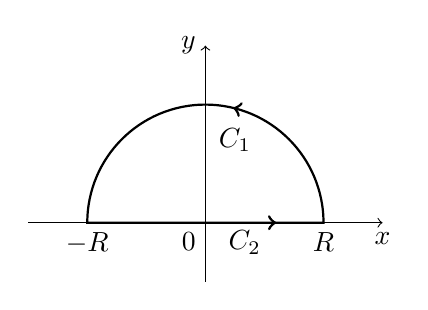
\begin{tikzpicture}[
            scale=0.75,
            decoration={markings,
            mark=at position 2.4cm with {\arrow[line width=1pt]{>}},,
            mark=at position 5cm with {\arrow[line width=1pt]{>}},
            }]
            % The axes
            \draw[->] (-3,0) -- (3,0) coordinate (xaxis);
            \draw[->] (0,-1) -- (0,3) coordinate (yaxis);

            % The path
            \path[draw,line width=0.8pt,postaction=decorate] (-2,0) node[below] {$-R$} -- (2,0) node (R) [below] {$R$} arc (0:180:2) -- (-1,0);

            % The labels
            \node[below] at (xaxis) {$x$};
            \node[left] at (yaxis) {$y$};
            \node[below left] {$0$};
            \node at (0.5,1.4) {$C_1$};
            \node[left of=R] {$C_2$};
        \end{tikzpicture}
    \end{minipage}
    \hfill
    \begin{minipage}{0.6\textwidth}
        \begin{equation*}
            \int_{C_R} f(z)\ dz = \int_{C_1} f(z)\ dz + \int_{C_2} f(z)\ dz
        \end{equation*}
        By the ML inequality,
        \begin{equation*}
            \left| \int_{C_2} f(z)\ dz \right| = \frac{R^2+1}{(R^2-\pi)(R^2-\pi/2)} (\pi R),\ R \to \infty,\ \text{RHS} \to 0
        \end{equation*}
    \end{minipage}
    Then $\int_{C_R} f(z)\ dz = \int_{-R}^R f(x)\ dx$ by definition of a contour integral. By the residue theorem,
    \begin{align*}
        \lim_{R \to \infty} \int_{C_R} f(z)\ dz = 2 \pi i \left[ \text{Res}_{i\sqrt{\pi}} f(z) + \text{Res}_{i\sqrt{\pi/2}} f(z) \right] = \frac{2}{\sqrt{\pi}} (\sqrt{2}-1)\left( \frac{\pi}{\sqrt{2} + 1} \right)
    \end{align*}
    Therefore,
    \begin{equation*}
        \int_0^\infty f(x)\ dx = \frac{1}{\sqrt{\pi}} (\sqrt{2}-1)\left( \frac{\pi}{\sqrt{2} + 1} \right)
    \end{equation*}
\end{example}

\begin{example} \normalfont
    \hl{(Improper integrals of trig fns).} We wish to evaluate integrals of the form
    \begin{equation*}
        \int_{-\infty}^\infty r(x) \begin{Bmatrix} \cos x \\ \sin x \end{Bmatrix}\ dx,\quad r(x)\ \text{is a rational fn.}
    \end{equation*}
    Notice that
    \begin{equation*}
        \int_{-\infty}^\infty r(x)e^{ix}\ dx = \int_{-\infty}^\infty r(x) \cos x\ dx + i \int_{-\infty}^\infty r(x) \sin x\ dx
    \end{equation*}
\end{example}

\begin{example} \normalfont
    Evaluate
    \begin{equation*}
        \int_0^\infty \frac{\cos 2x}{x^2+4}\ dx
    \end{equation*}
    We take the same contour as in Example \ref{ex:contour}. Then,
    \begin{align*}
        \Im \left( \lim_{R \to \infty} \int_{C_2} f(z)\ dz \right) &= \int_{-\infty}^\infty \frac{\cos 2x}{x^2+4}\ dx \\
        \left| \int_{C_1} f(z)\ dz \right| &\leq \left| \frac{e^{2iz}}{z^2+4} \right|\ |dz| \leq \frac{1}{R^2+4} (\pi R) \xrightarrow{R \to \infty} 0
    \end{align*}
    By residue theorem,
    \begin{equation*}
        \int_{C_R} \frac{e^{2iz}}{z^2+4} = 2 \pi i \text{Res}_{2i} f(z) = 2 \pi i \lim_{z \to 2i} \frac{e^{2iz}}{z+2i} = \frac{\pi}{2e^4}
    \end{equation*}
    Therefore,
    \begin{equation*}
        \int_0^\infty \frac{\cos 2x}{x^2 + 4}\ dx = \frac{\pi}{4} e^{-4}
    \end{equation*}
\end{example}

\begin{remark} \normalfont
    CAUTION:
    \begin{equation*}
        \lim_{R \to \infty }\left| \int_{C_1} \frac{\cos 2x}{x^2+4}\ dz \right| \neq 0,\quad \text{b/c $\cos 2x$ is not an odd fn.}
    \end{equation*}
\end{remark}

\begin{example} \normalfont
    \hl{(Definite integrals of trig fns).}
    \begin{equation*}
        \int_0^{2\pi} F(\cos \theta, \sin \theta)\ d\theta = \oint_{|z|=1} F\left( \frac{z+z^{-1}}{2}, \frac{z-z^{-1}}{2i} \right)\ \frac{dz}{iz} = 2 \pi i \text{Res}_{p \in \{ |z| < 1 \}} \frac{F}{iz}
    \end{equation*}
    CAUTION: Don't forget to divide by $i$ when converting the sin term and computing the residue!
\end{example}

\begin{example} \normalfont
    Let $-1 < a < 1$ and $a \neq 0$. Evaluate
    \begin{equation*}
        \int_0^{2\pi} \frac{d\theta}{1 + a \cos \theta}
    \end{equation*}
    We compute
    \begin{align*}
        \int_0^{2\pi} \frac{d\theta}{1 + a \cos \theta} &= \int_{|z|=1} \frac{1}{1+a \left( \frac{z+z^{-1}}{2} \right)} \frac{dz}{iz} = \int_{|z|=1} \frac{dz}{z^2 + 2z/a + 1} \\
        \intertext{Roots of denominator: $z = \left\{ z_1 = -\frac{1}{a} + \frac{1}{a} \sqrt{1-a^2}, z_2 = -\frac{1}{a} - \frac{1}{a} \sqrt{1-a^2} \right\}.$ Only $z_1$ is inside $|z| = 1$.}
        \implies \int_0^{2\pi} \frac{d\theta}{1 + a \cos \theta} &= 2 \pi i \frac{2}{ia} \text{Res}_{z_1} \frac{1}{z^2 + 2z/a + 1} = \frac{2 \pi}{\sqrt{1-a^2}}
    \end{align*}
\end{example}

\section{Laplace Transform}

\begin{definition}
    The Laplace transform is defined as
    \begin{equation*}
        \mathcal{L}(f(t)) = F(s) = \int_0^\infty e^{-st} f(t)\ dt
    \end{equation*}
\end{definition}

\begin{theorem} \label{thm:inv-laplace}
    (Inverse Laplace transform). Let $s \in \mathbb{C}$ be a complex variable and $f$ be a real-valued function in domain $t \geq 0$. Assume $f$ is piecewise continuous and exponentially bounded. Then
    \begin{equation*}
        f(t) = \mathcal{L}^{-1} (F(s)) = \frac{1}{2 \pi i} \int_{k-i\infty}^{k+i\infty} F(s) e^{st}\ ds
    \end{equation*}
    By residue theorem,
    \begin{equation*}
        f(t) = \mathcal{L}^{-1} (F(s)) = \sum_{p:\ F(s) \text{ singular at } p} \text{Res}_p(F(s)e^{st})
    \end{equation*}
    Furthermore,
    \begin{equation*}
        f(t) = \mathcal{L}^{-1} (F(s)) = \text{Res}_{w=0} \frac{1}{w^2} e^{t/w} F \left( \frac{1}{w} \right)
    \end{equation*}
\end{theorem}

\begin{example} \normalfont
    Find the inverse Laplace transform of
    \begin{equation*}
        F(s) = \frac{s}{(s+1)(s-1)^2}
    \end{equation*}
    Apply theorem \ref{thm:inv-laplace}.
    \begin{align*}
        F(s) e^{st} &= \frac{se^{st}}{(s+1)(s-1)^2} \\
        \text{Res}_{-1} \frac{se^{st}}{(s+1)(s-1)^2} &= -\frac{e^{-t}}{4} \\
        \text{Res}_1 \frac{se^{st}}{(s+1)(s-1)^2} &= \left. \frac{2 \pi i}{1!} \frac{d}{ds} \left( \frac{se^{st}}{s+1} \right) \right\rvert_1 = \frac{(1+2t)e^t}{4} \\
        f(t) &= -\frac{e^{-t}}{4} + \frac{(1+2t)e^t}{4}
    \end{align*}
\end{example}

\end{document}
